
\section{CHAPTER 3: STEAM ENGINEERING}
\subsection{What is Steam?}
Steam is the gas formed when water passes from the liquid to the gaseous state.
At the molecular level, this is when $H_2O$ molecules manage to break free from the bonds 
(i.e. hydrogen bonds) keeping them together\cite{what_is_steam}\relax.


\subsection{Types of Steam:}
When water is heated to its boiling point, it transforms into steam. The temperature at which this transformation occurs is known as the boiling point. The boiling point of water is 100°C at atmospheric pressure. However, the boiling point of water changes with pressure. For example, at a pressure of 10 bar, the boiling point of water is 180°C. The relationship between pressure and temperature is illustrated in Figure \ref{fig:ptrws}.

\begin{figure}[h!]
    \centering
    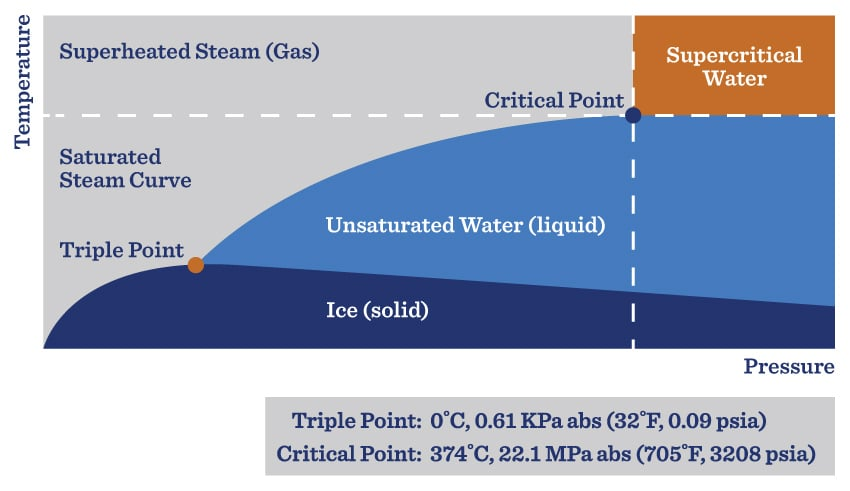
\includegraphics[width=\linewidth]{figs/steam.jpg}
    \caption{Pressure-Temperature Relationship of Water \& Steam}
    \label{fig:ptrws}
\end{figure}
Depending on the pressure, temperature, content of water different types of steam are produced. The most common types of steam are:

\textbf{1. Dry steam:} All its water molecules remain in the gaseous state. Hence, it's a transparent gas\cite{steam_types_tlv}.

\textbf{2. Wet steam:} A portion of its water molecules have given up their energy (latent heat) and condense to form tiny water droplets. Hence, these droplets make the steam look white and opaque\cite{steam_types_tlv}.

\textbf{3. Saturated Steam:} - Application Area: Indirect Heating - Process Application.
Saturated steam refers to steam that is completely dry and has the same temperature as the water from which it is formed. When water is boiled, its temperature increases until it reaches the boiling point at that pressure.

If additional heat is applied to the water, it converts to steam by absorbing the latent heat of evaporation. This steam, which exists at the same temperature as the water, is known as saturated steam. If saturated steam does not contain any water droplets, it is called dry saturated steam\cite{steam_types_fm}.

\textbf{4. Vacuum Steam:}
As we know, at a specific pressure, saturated steam always exists at the boiling point of water at that pressure. Saturated steam exists at approximately 100°C at atmospheric pressure. 
If the pressure is reduced, the temperature at which saturated steam is formed also decreases. This steam, generated under sub-atmospheric pressure (vacuum conditions), is called vacuum steam. Vacuum steam has a temperature below 100°C\cite{steam_types_fm}.

\textbf{5. Superheated Steam:} - Application Area: Power Generation. If saturated steam is further heated, its temperature continues to rise above the boiling point. Such steam, with a temperature higher than the boiling point at that pressure, is referred to as superheated steam\cite{steam_types_fm}.

\textbf{6. Clean Steam:} - Application Area: Injection (Direct Heating). Clean steam is steam that is free from impurities. It is generated using a clean steam generator. Clean steam is used in the pharmaceutical industry for injection purposes. It is also used in the food industry where steam comes into direct contact with the food product\cite{steam_types_fm}.

\subsection{Steam As a Source of Heat}
Steam played a crucial role in the industrial revolution. However, in modern times, steam has been largely replaced by internal combustion engines and electricity as a power source. Nowadays, steam is primarily recognized for its applications in heating, serving as both a \textbf{direct} and \textbf{indirect} source of heat.

The concept behind using steam for cooking is that when steam comes into direct contact with the food being heated, the latent heat of steam is directly transferred to the food, while the condensation of water droplets provides moisture.

In industrial processes, direct steam heating is commonly employed for cooking, sterilization, steam smothering, vulcanization, and other procedures.

On the other hand, indirect steam heating refers to processes where steam does not directly contact the product being heated. This method is widely utilized in industry due to its ability to provide rapid and uniform heating. Typically, a heat exchanger is used to heat the product in this method.

One advantage of indirect steam heating over direct steam heating is that the formation of water droplets during heating does not affect the product. As a result, steam can be utilized in various applications such as melting, drying, and boiling.

Indirect steam heating finds extensive use in processes related to the production of food and beverages, tires, paper, cardboard, fuels like gasoline, and pharmaceuticals, among others.

\subsection{Parts of Steam Engineering}
\begin{enumerate}
    \item \textbf{Boiler}: A vital part of the system, the boiler heats water to produce steam. Usually, it includes a combustion chamber, furnace, tubes, and a number of temperature and pressure control devices. 
    \item \textbf{Steam turbine}: High-pressure steam's thermal energy is transformed into mechanical energy using a steam turbine. It has a rotor with blades that the high-velocity steam rotates, creating power. 
    \item \textbf{Condenser}: By cooling down the turbine's exhaust steam, the condenser is in charge of transforming it back into liquid form. By producing a vacuum that allows steam to be used more effectively. 
    \item \textbf{Piping System}: Steam is transported from the boiler to the target destination via a pipe system called steam piping. To provide a secure and effective flow of steam, it contains pipes, fittings, valves, and insulation. 
    \item \textbf{Pressure Reducing Valve}: A pressure-reducing valve is used to regulate and lower the pressure of steam from high levels to lower, safer levels appropriate for a variety of applications. 
    \item \textbf{Steam control valves}: These valves control steam flow to manage pressure and temperature. They are essential for preserving the best process conditions and guaranteeing safe operation. 
    \item \textbf{Steam Traps}: Steam traps are used to get rid of the condensate (water) that builds up in the steam system. They guarantee that heat is transferred effectively and help prevent water from building up in the pipes. 
    \item \textbf{Steam Condensate Recovery System}: Condensate (condensed steam) is collected and returned to the boiler by the steam condensate recovery system. It lowers operating expenses and aids in energy and water conservation. 
    \item \textbf{Safety Valves}: Vital parts that guard the system from overpressure include safety valves. In order to avoid catastrophic failures or equipment damage, they automatically expel excess steam.
    \item \textbf{Instrumentation and controls:} To monitor and manage steam characteristics like temperature, pressure, flow rate, and level, steam engineering needs a variety of instruments and control systems. These consist of sensors, gauges for measuring pressure and temperature, and automation systems. 
\end{enumerate} 


\subsection{Application of Steam}
There are many industry verticles wheere steam is used, below are some of the areas where steam is used extensively.
\begin{enumerate}
    \item Textile industry
    \item Food \&\ Beverage industry
    \item Ceremic industry
    \item Sugar industry
    \item Pulp industry
    \item Dairy industry
\end{enumerate}